\subsection{Muon system trigger rates}
\label{sec:muontrigg}

As in the case of ECal, trigger rates in the muon system are dominated by the beam background. In order to estimate the rates, GEANT4 model of the HPS detector was used where the muon system is described according to the conceptual design presented in Section\ref{sec:muon}. Figure \ref{fig:HPS_view2} shows layout of the system. Each of eight hodoscope layers (four layers in the top part of the detector and four in the bottom) consists of two planes of scintillator strips. In one of planes strips are oriented horizontally, so called Y-plane. In the second, called X-plane, they are oriented vertically. For the readout purposes, the Y-planes are segmented into two parts, left and right (cut exactly at the geometrical mid point of the plane) and each half plane is composed of three strips. The total number of Y-strips is 48. X-planes are divided into 4.5 cm wide segments, with 240 strips in total. It should be noted that the number of vertical strips in the conceptual design is only 208. As will be discussed below rates in the vertical strips at the edges of hodoscope planes are very low and eight strips in each plane can be paired to make four readout channels without any impact on the detector occupancy. In Table \ref{tb:muonstrp}, lengths and widths of the detector readout segments (counters) are presented. There is a $14$ cm wide and $3.5$ cm high gap introduced into the model, centered at electron beam direction, to avoid high rate region. As shown in Figure \ref{fig:xymu} this gap will have negligible effect on the muon pair detection efficiency from $\ap$ decays. 

\begin{table}[htdp]
\caption{Lengths and widths of the hodoscope strips. Dimensions are centimeters.}
\begin{center}
\begin{tabular}{|c|c|c|c|c|}
\hline\hline
Readout plane& Layer 1&Layer 2&Layer 3& Layer 4 \\
\hline
X-plane width& 4.5& 4.5 & 4.5 & 4.5  \\
X-plane length&10.5&11.5&12.5&13.5\\
\hline
Y-plane width& 3.5 all three&3.5, 4, 4  & 3.5, 4.5, 4.5 & 4.5 all three\\
Y-plane length&56&62.5&70&76\\
\hline\hline
\end{tabular}
\end{center}
\label{tb:muonstrp}
\end{table}%

As an input to GEANT4 detector simulator, events generated in EGS5 were used. The CEBAF beam bunch structure was simulated by sending one bunch 
equivalent of electrons, 5,625 $e^-$'s (6.6 GeV), through 
the target. The produced secondaries were sent throug the GEANT4 model to simulate detector response. As it was expected, the highest rates are detected in Layer 1 hodoscope and are on order of $\sim 0.7$ MHz (X-strips at the electron beam location and the beam-left Y-strip closest to the beam plane), see Figure \ref{fig:l1rates}. Rates in the vertical strips far a way from the beam position are very low and the multiple strips can be combined into a single readout channels in order to reduce the number of PMTs and the electronic channels.  

\begin{figure}[htbp]
\begin{center}
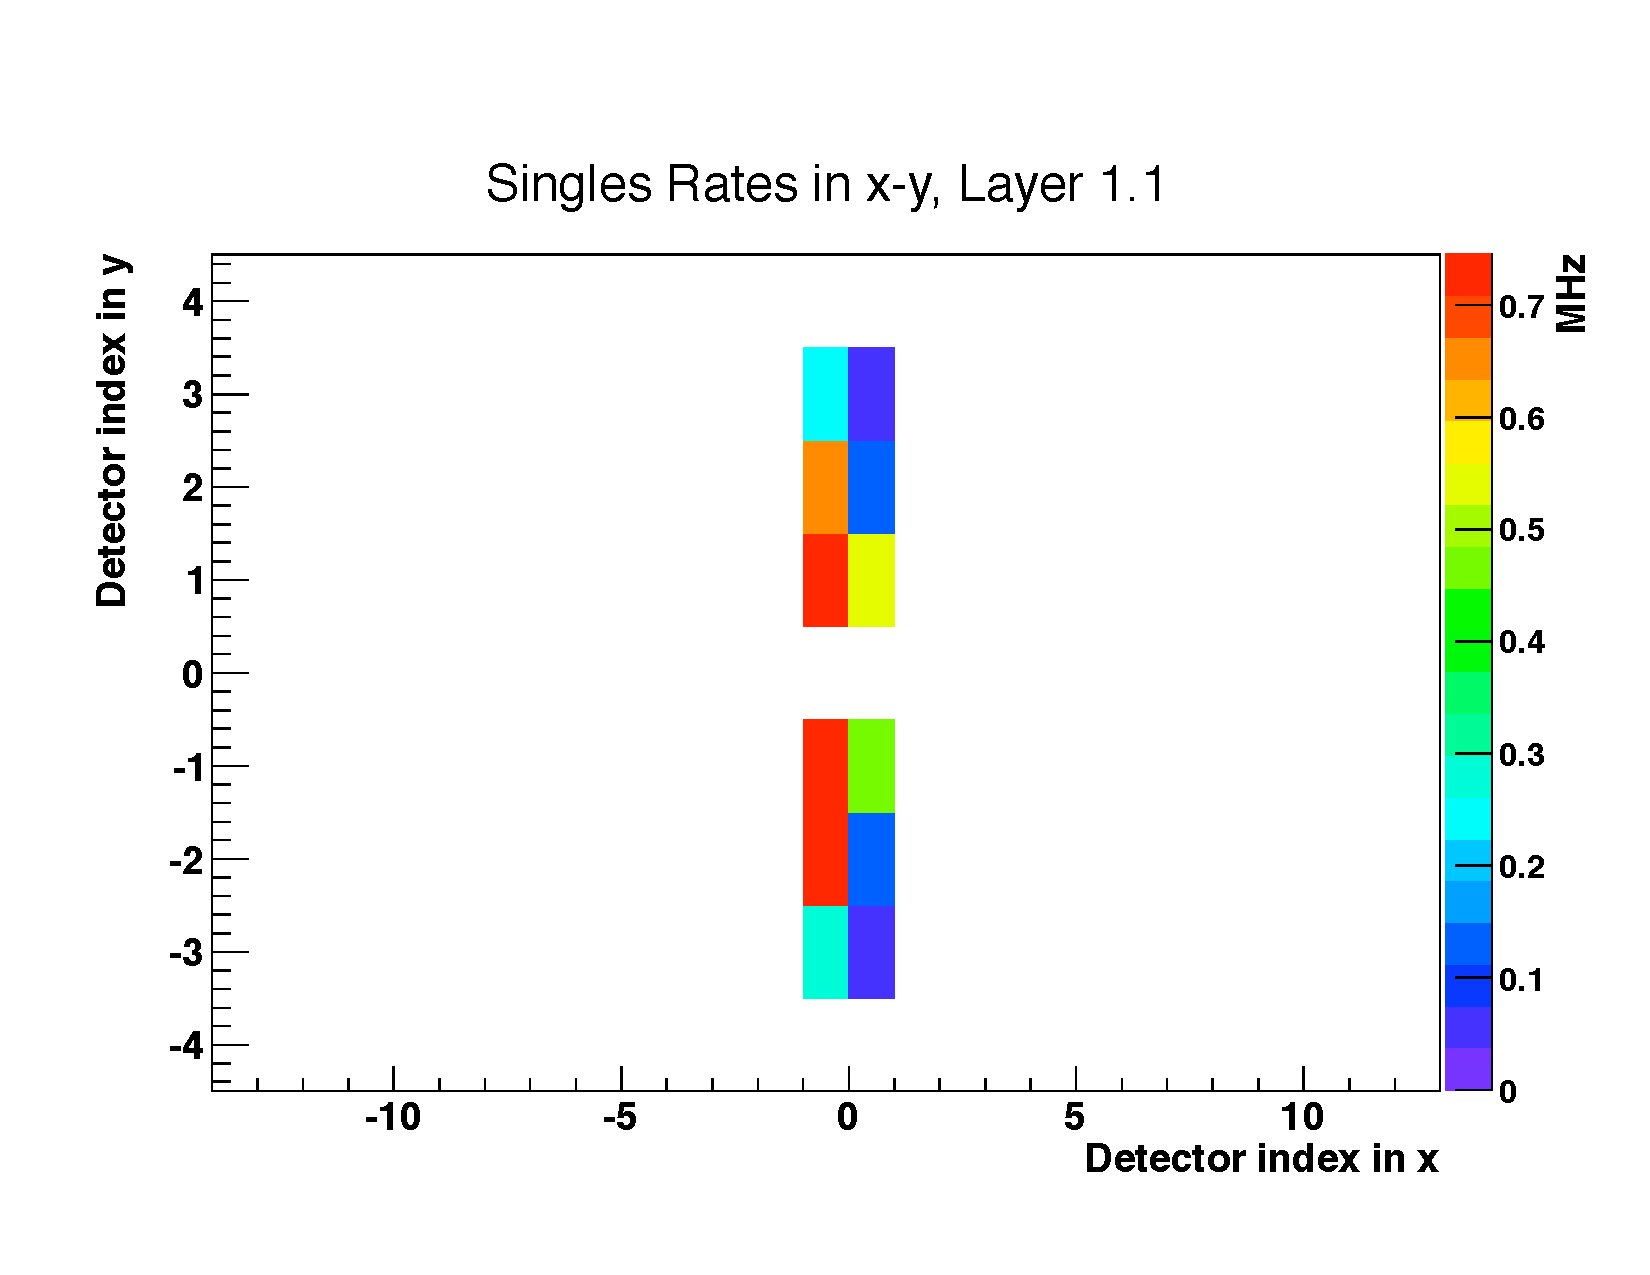
\includegraphics[width=0.475\textwidth]{performance/trigger/muon_singles1}
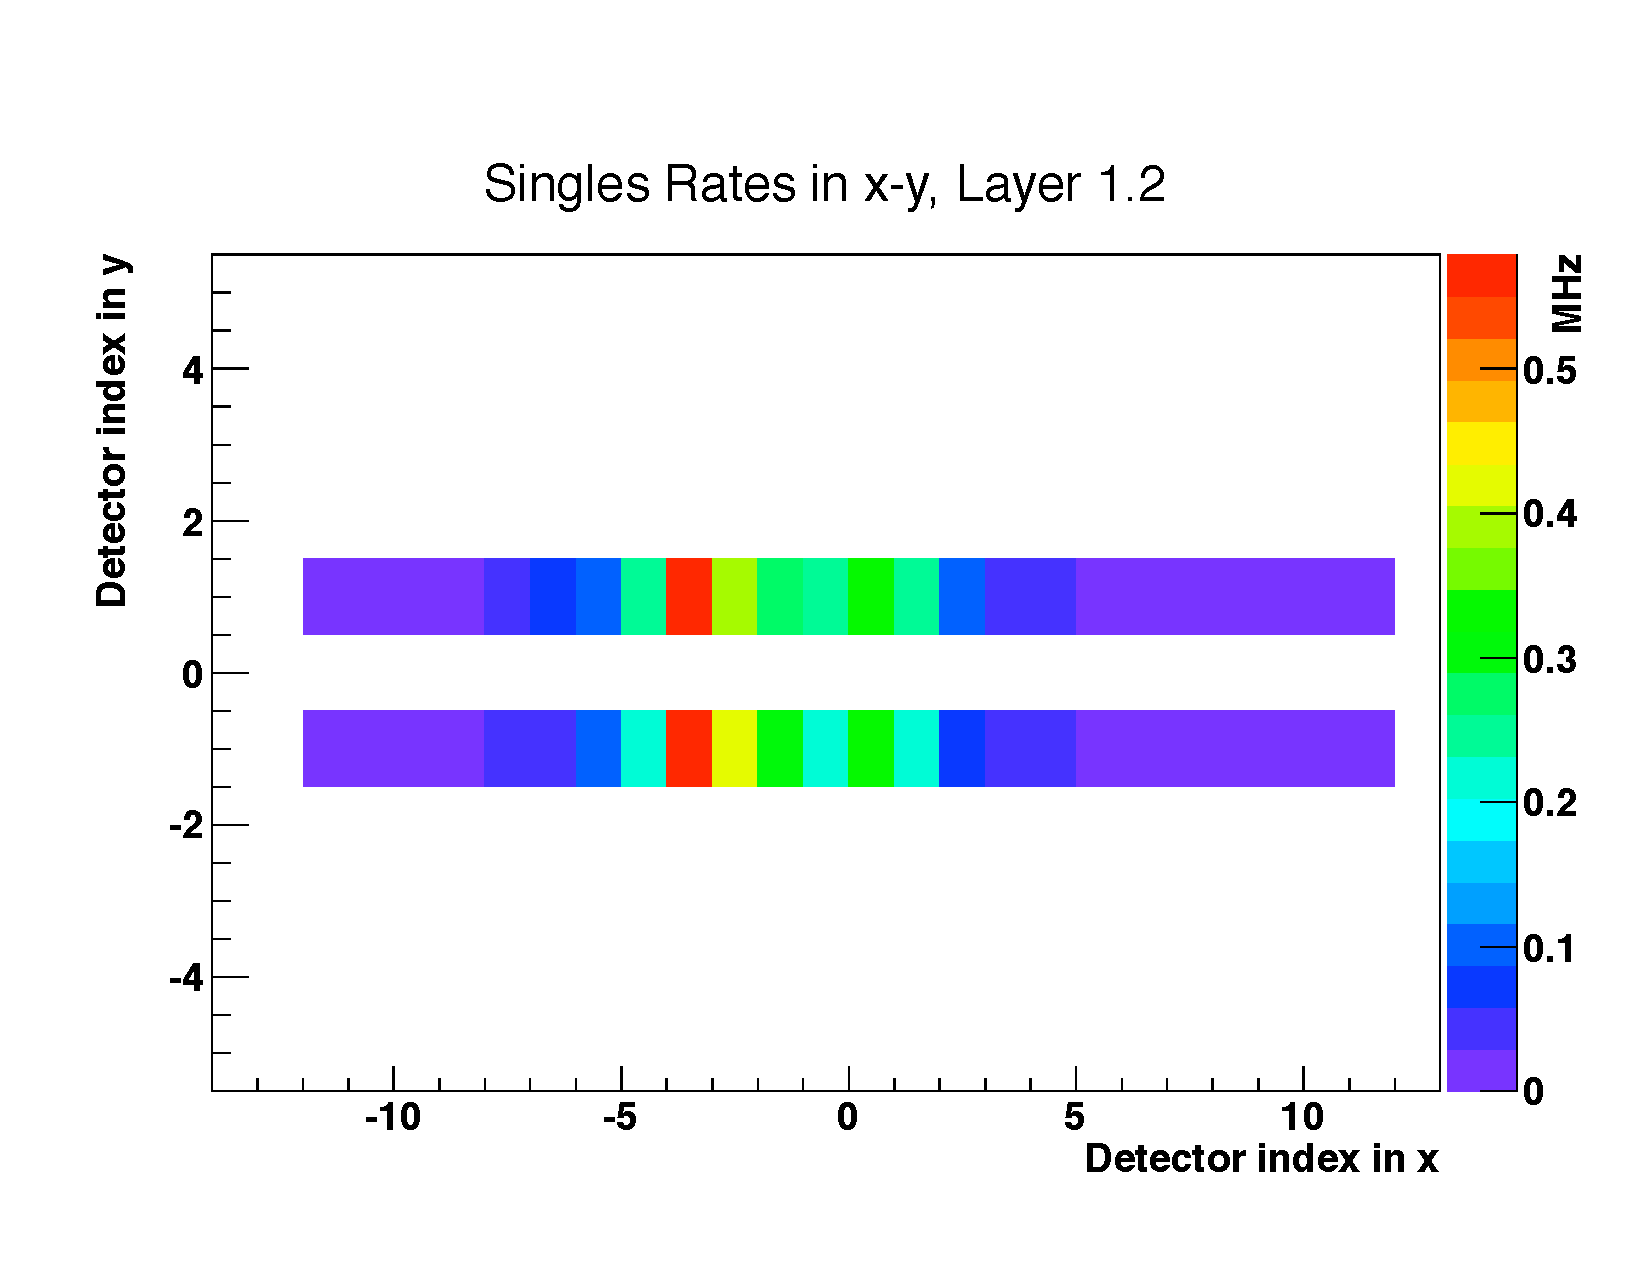
\includegraphics[width=0.475\textwidth]{performance/trigger/muon_singles2}
\caption{Rates in Y- (left) and X-planes (right) of the Layer 1 hodoscopes for hits with energy deposition $> 0.5$ MeV.}
\label{fig:l1rates}
\end{center}
\end{figure}

The coincidence rates between hodoscope planes in a layer and between layers have been studied using a $16$ ns coincidence time window. In the left graph of  Figure \ref{fig:c1rates} coincidence rates between X- and Y-quadrants (top-left, top-right, bottom-left, and bottom-right) of Layer 1 hodoscope are shown. The right graph of the figure shows coincidence rates of respective quadrants of Layers 1 and 2. For the muon trigger, a coincidence of the first three layers of hodoscopes is required. The rates of the triple coincidence within $16$ ns are shown in Figure \ref{fig:c3rates}. The maximum trigger rates are in the beam-left quadrants and is on order of $7$ kHz. While further reduction of rates will be possible with inclusion of MIP hits in ECal, the $7$ kHz is already within the limit of allowed rate for HPS DAQ.   

\begin{figure}[htbp]
\begin{center}
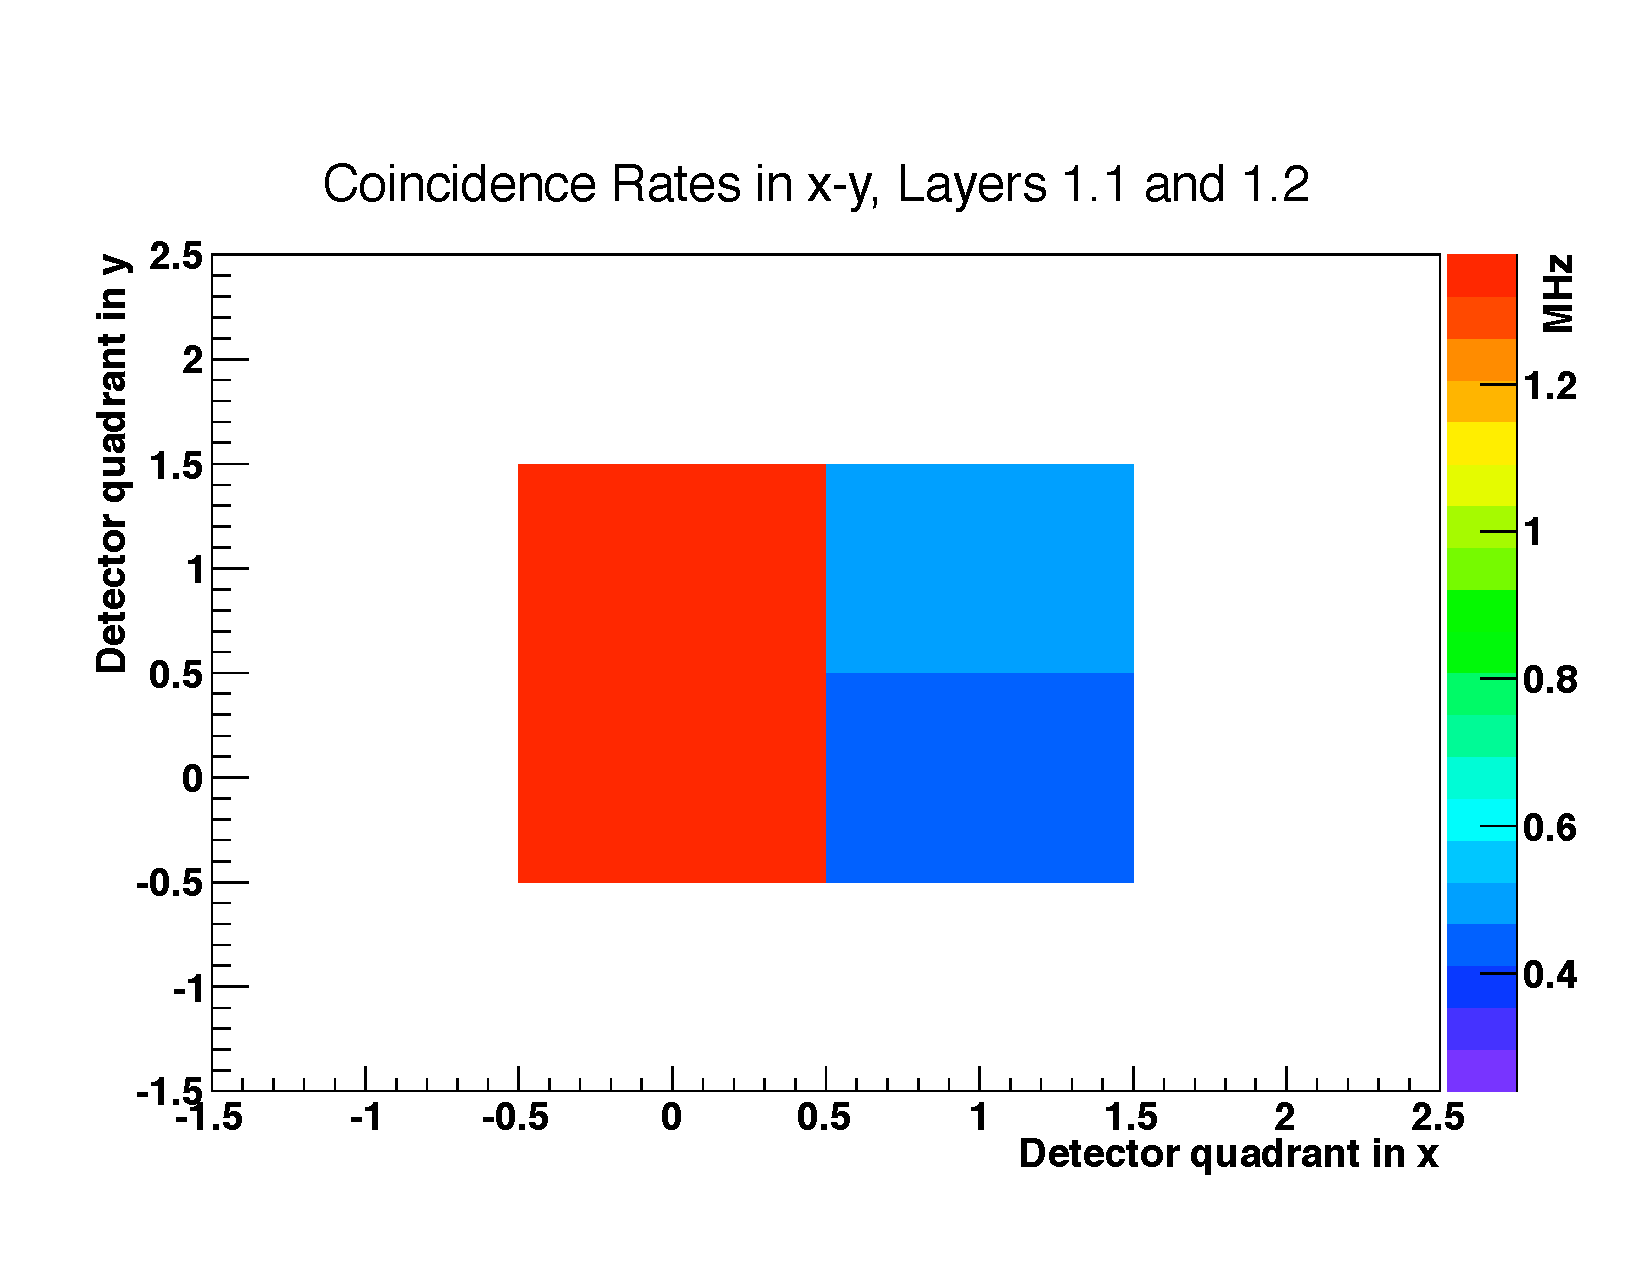
\includegraphics[width=0.475\textwidth]{performance/trigger/muon_coinrate1}
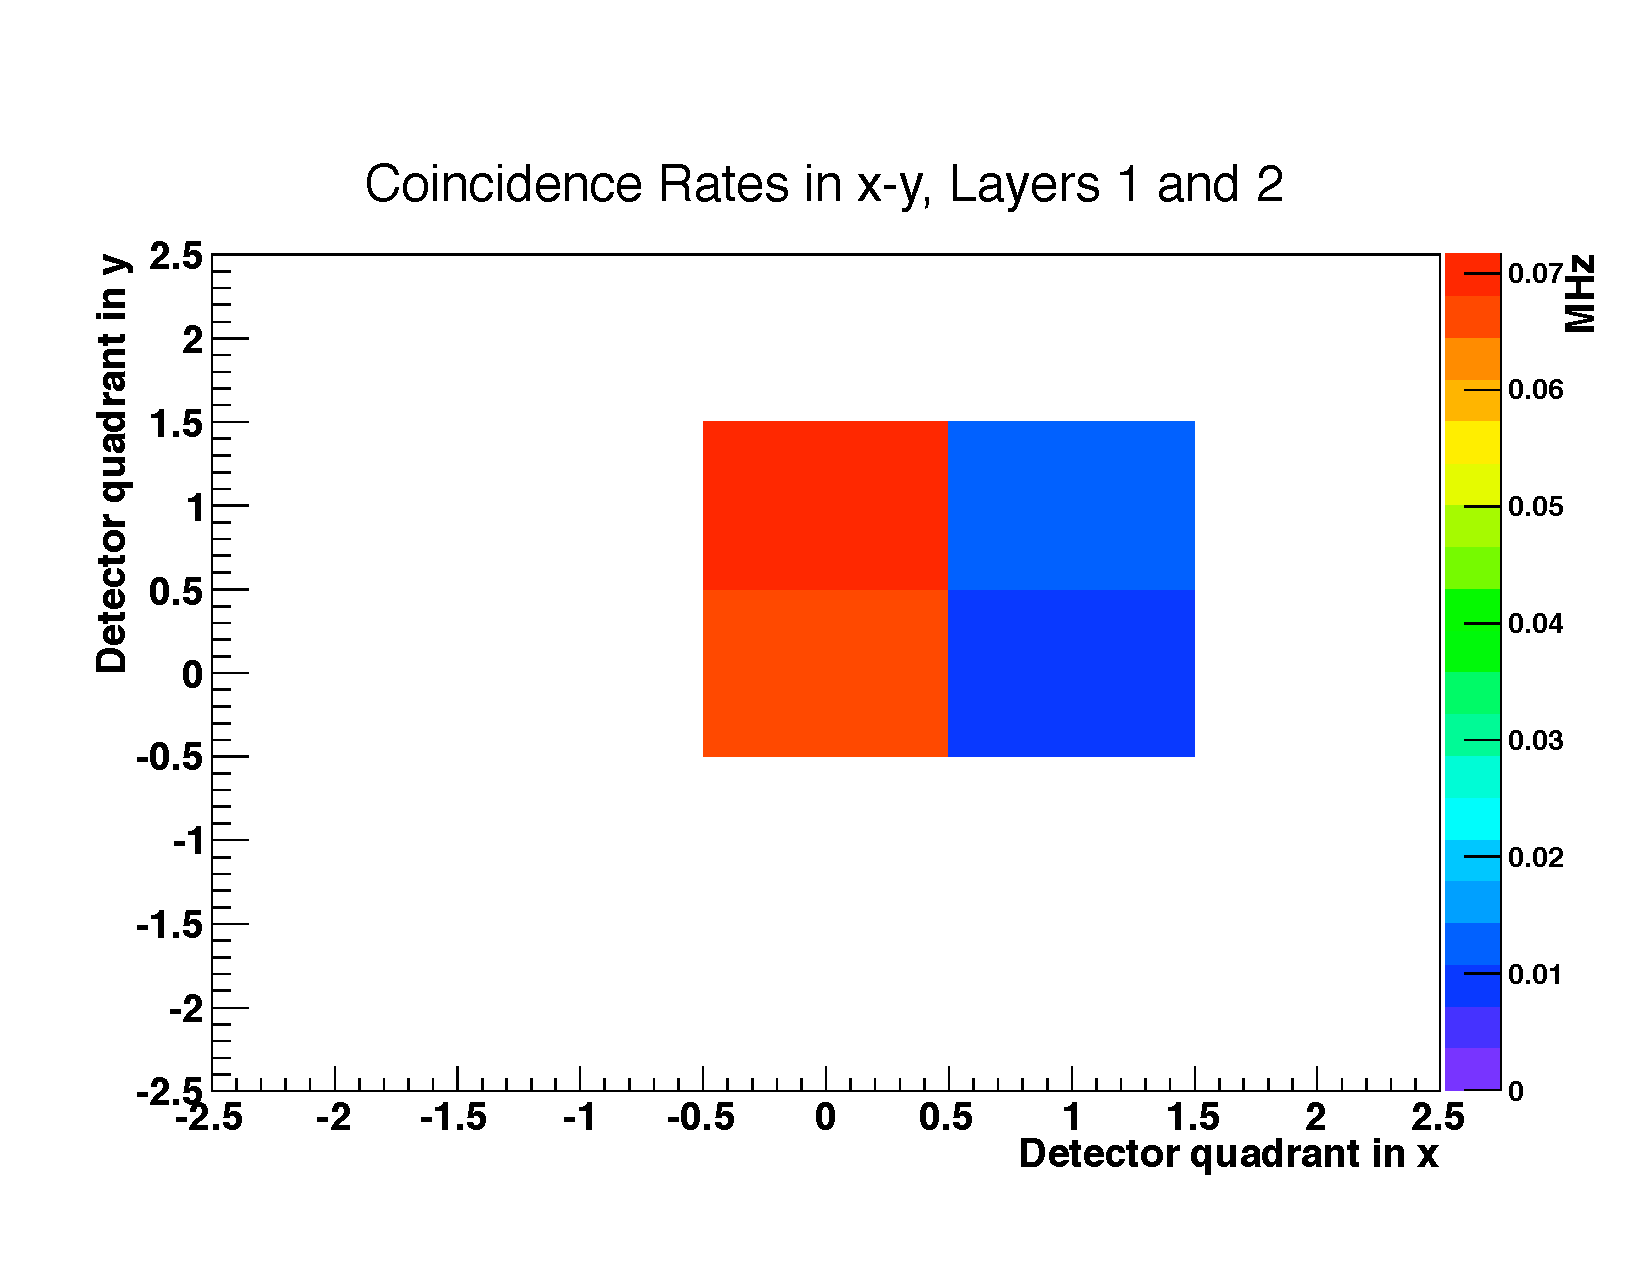
\includegraphics[width=0.475\textwidth]{performance/trigger/muon_coinrate2}
\caption{Coincidence rates between X- and Y-quadrants of the Layer 1 hodoscope (left graph) and coincidence rates between Layer 1 and 2 (right graph). }
\label{fig:c1rates}
\end{center}
\end{figure}

\begin{figure}[htbp]
\begin{center}
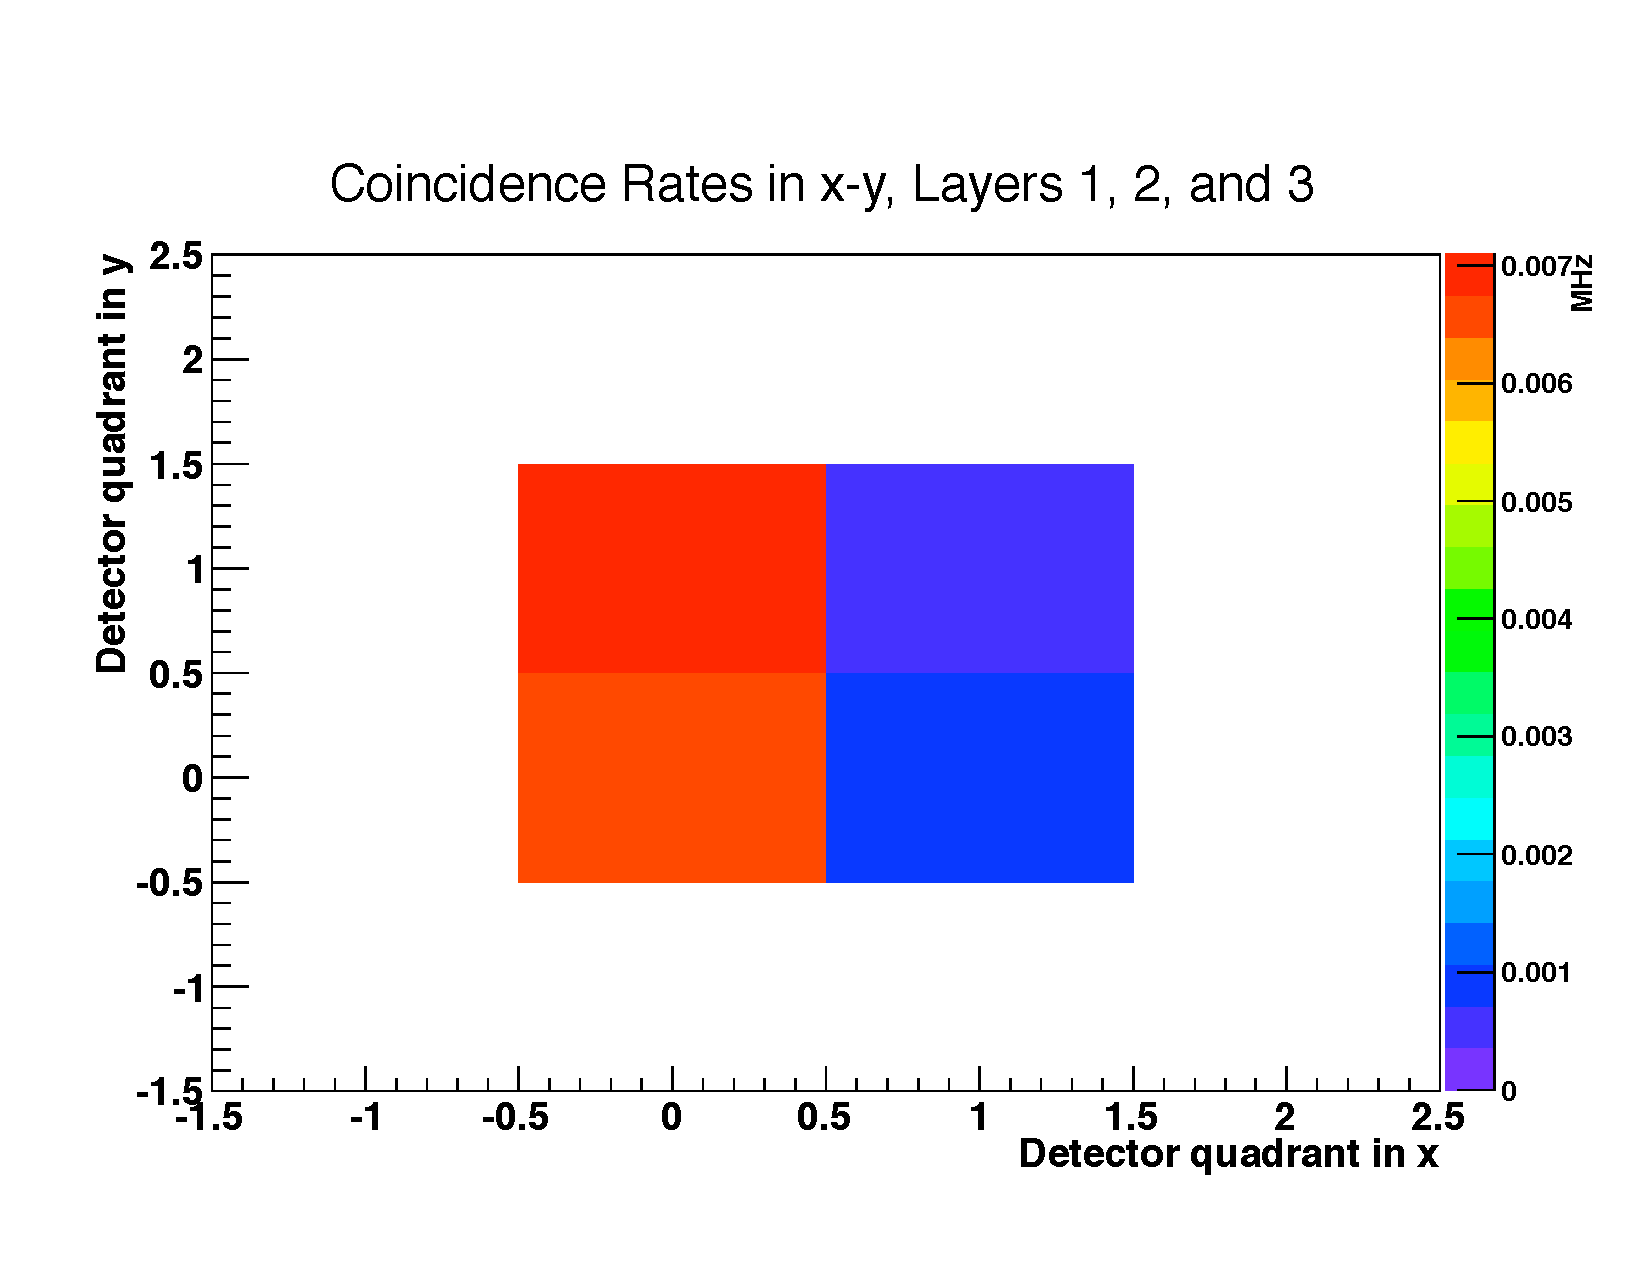
\includegraphics[width=\textwidth]{performance/trigger/muon_coinrate3}
\caption{Coincidence rates in first three layers of muon hodoscopes. The coincidence time window is set to $16$ ns. }
\label{fig:c3rates}
\end{center}
\end{figure}





